\documentclass[10pt,twocolumn,a4paper]{article}

\usepackage[utf8]{inputenc}
\usepackage[T1]{fontenc}
\usepackage{lmodern}
\usepackage[spanish,es-tabla,es-noshorthands]{babel}
\usepackage[margin=1.8cm,columnsep=0.6cm]{geometry}
\usepackage{amsmath,amssymb}
\usepackage{icomma}
\usepackage{graphicx}
\usepackage{booktabs}
\usepackage[numbers,sort&compress]{natbib}
\usepackage[hidelinks]{hyperref}

% Las figuras viven en ../figuras dentro del repositorio; en Overleaf, subirlas
% a una carpeta figuras/ al lado de este archivo.
\graphicspath{{../figuras/}{figuras/}}

\newcommand{\etaT}{\eta_T}
\newcommand{\etaL}{\eta_L}

\title{\Large Combinar o reentrenar: aprendizaje online con \emph{Hedge}\\
para detección de spam bajo ataque adversarial}
\author{Pablo Díaz \qquad Ezequiel Martinez\\
\small Tópicos Avanzados en Ciencia de Datos (MCD210) --- Maestría en Ciencia de Datos, UdeSA}
\date{Septiembre 2026}

\begin{document}

\twocolumn[
\begin{@twocolumnfalse}
\maketitle
\begin{abstract}
Un filtro de spam enfrenta a un adversario que adapta sus mensajes para evadirlo. Ante eso hay dos
remedios que la formulación usual mezcla: \emph{combinar} clasificadores fijos con pesos que se
reacomodan (\emph{Hedge}) o \emph{reentrenar} un único modelo con los datos que llegan. Los separamos
sobre el SMS Spam Collection con un ataque de ofuscación léxica que reduce a la mitad la detección
de un filtro bayesiano. Con todas las etiquetas, reentrenar recupera más, pero \emph{Hedge} cubre el
$47 \pm 13\,\%$ de la brecha sin tocar ningún modelo. Cuando las etiquetas escasean el orden se
invierte: con 5\,\% de mensajes etiquetados, combinar gana en 16 de 20 semillas. De paso mostramos
que la cota de la teórica corresponde al \emph{Hedge} randomizado y no al voto pesado
determinístico, que admite regret lineal, y que cada cota vale solo para su propia tasa de
aprendizaje.
\end{abstract}
\vspace{1em}
\end{@twocolumnfalse}
]

% ---------------------------------------------------------------------------
\section{Introducción}

La detección de spam es un problema adversarial: el spammer observa qué pasa y qué no pasa el
filtro, y adapta sus mensajes~\cite{fraiman2026clase2}. \citet{lowd2005goodword} mostraron que
agregando unas pocas decenas de palabras típicas del correo legítimo la mitad del spam bloqueado
logra pasar, y concluyeron que \emph{``the only remedy we know of is frequent retraining''}.

El aprendizaje online ofrece otra respuesta. \emph{Hedge}~\cite{freund1997decision} mantiene pesos
exponenciales sobre $K$ clasificadores fijos y garantiza cometer casi tan pocos errores como el
mejor de ellos en retrospectiva, sin supuestos estadísticos sobre la secuencia. La propuesta de la
materia compara \emph{Hedge} contra un modelo estático, pero no contra el remedio clásico de
reentrenar, y así no distingue si lo que ayuda es \emph{combinar} expertos o simplemente
\emph{adaptarse}. Este trabajo separa los dos efectos y responde dos preguntas:
\begin{enumerate}
\item ¿Cuánto de la recuperación frente al ataque se obtiene combinando expertos congelados, sin
reentrenar nada?
\item ¿Cuánta etiqueta hace falta? En la práctica el usuario reporta solo algunos mensajes.
\end{enumerate}
En el camino aparecen tres precisiones sobre la teórica que el trabajo desarrolla: el algoritmo y la
cota que se presentan juntos corresponden a procedimientos distintos (\S\ref{sec:det}); cada cota
vale solo para su tasa de aprendizaje (\S\ref{sec:marco}); y el \emph{feedback} tipo bandit no
aporta nada en este problema (\S\ref{sec:rho}).

% ---------------------------------------------------------------------------
\section{Marco formal}\label{sec:marco}

En cada ronda $t = 1, \dots, T$ llega un mensaje $x_t$, el jugador predice $\hat y_t \in \{0,1\}$,
se revela $y_t$ y se sufre $\mathbb{1}\{\hat y_t \neq y_t\}$. Los $K$ expertos son funciones fijas
$f^{(i)}$, entrenadas sobre un tramo inicial (\emph{warm-up}) y congeladas; su pérdida es
$\ell_t(i) = \mathbb{1}\{f^{(i)}(x_t) \neq y_t\}$. El regret compara contra el mejor experto fijo en
retrospectiva:
\begin{equation}
R_T = \sum_{t=1}^{T} \mathbb{1}\{\hat y_t \neq y_t\} - \min_i \sum_{t=1}^{T} \ell_t(i).
\end{equation}
El adversario es \emph{oblivious}: fija la secuencia de antemano. La elección no es de comodidad:
contra un adversario que reacciona a las jugadas, esta definición de regret deja de tener sentido y
hace falta \emph{policy regret}, y sin acotar su memoria el regret lineal es inevitable para
cualquier algoritmo~\cite{cesabianchi2013switching,arora2012online}.

\emph{Hedge} actualiza $w_{t+1}(i) \propto w_t(i)\, e^{-\eta\, \ell_t(i)}$ desde pesos uniformes y
juega la predicción de un experto sorteado $I_t \sim w_t$. Con $\eta$ fijo, el lema de Hoeffding da,
para toda ronda $t$,
\begin{equation}\label{eq:peorcaso}
\mathbb{E}[R_t] \le \frac{\ln K}{\eta} + \frac{\eta\, t}{8},
\end{equation}
que con $\etaT = \sqrt{8 \ln K / T}$ vale $\sqrt{T \ln K / 2}$ en $t = T$ (la $\sqrt{2T\ln K}$ de
la teórica es el doble: correcta pero conservadora). \citet{freund1997decision} dan además una cota
en función de la pérdida $L_i(t)$ de cualquier experto:
$\mathbb{E}[L_{\text{Hedge}}(t)] \le (\ln K + \eta\, L_i(t))/(1 - e^{-\eta})$. Con
$\etaL = \ln\!\big(1 + \sqrt{2\ln K / L_{\text{best}}}\big)$ se obtiene
$R_T \le \sqrt{2 L_{\text{best}} \ln K} + \ln K$, que depende de la pérdida del mejor experto y no
del horizonte. Son dos configuraciones del mismo algoritmo y \textbf{cada cota vale solo para la
suya}; además $\etaL$ requiere conocer $L_{\text{best}}$ de antemano, lo que bajo drift es
información de oráculo.

% ---------------------------------------------------------------------------
\section{Algoritmos}

\subsection{Voto pesado determinístico o \emph{Hedge} randomizado}\label{sec:det}

La teórica presenta la predicción como voto pesado ($\hat y_t = 1$ si
$\sum_i w_t(i) f^{(i)}(x_t) > 1/2$) junto con la cota de \emph{Hedge}, que es la del jugador
randomizado. No es notación: un jugador determinístico no admite cota de regret sublineal, porque
aun un adversario \emph{oblivious} puede simularlo de antemano. Con dos expertos (uno dice siempre
``legítimo'', el otro siempre ``spam'') y etiquetas $y_t = 1 - \hat y_t$, el determinístico yerra
todas las rondas y el mejor experto la mitad: $R_T = T/2$ (Fig.~\ref{fig:regret}B). El randomizado,
sobre la misma secuencia, queda en $\approx 14$ con $T = 4000$, bajo su cota de 37.

\subsection{Etiqueta escasa, y por qué no EXP3}\label{sec:rho}

Para modelar que no se observan todas las pérdidas, lo natural sería EXP3~\cite{auer2002nonstochastic},
que solo ve la pérdida del experto jugado. Pero aquí ese \emph{feedback} colapsa en información
completa: los expertos son funciones conocidas de $x_t$, así que saber si la predicción jugada fue
correcta revela $y_t$, y con $y_t$ la pérdida de todos. La escasez real es otra: el usuario reporta
solo algunos mensajes. Modelamos que $y_t$ se observa con probabilidad $\rho$; en las rondas sin
etiqueta nadie actualiza, y en las observadas \emph{Hedge} usa el estimador insesgado $\ell/\rho$,
el mismo truco de EXP3. Como $\mathbb{E}[(\ell/\rho)^2] \le 1/\rho$, la técnica de
\citet{auer2002nonstochastic} da $\mathbb{E}[R_T] \le \ln K/\eta + \eta T/(2\rho)$; con
$\eta = \sqrt{\rho}\,\etaT$, el regret escala como $1/\sqrt{\rho}$.

\subsection{El competidor que reentrena}

Una regresión logística entrenada por SGD sobre el mismo \emph{hashing} que los expertos léxicos:
arranca entrenada sobre el \emph{warm-up}, en cada ronda predice primero y se actualiza después, y
con $\rho < 1$ solo se actualiza en las rondas etiquetadas (sin reponderar: aprende de los ejemplos
que tiene). A diferencia de \emph{Hedge}, puede aprender tokens que nunca vio.

% ---------------------------------------------------------------------------
\section{Diseño experimental}

\paragraph{Datos.} SMS Spam Collection~\cite{almeida2011contributions}: 5.574 mensajes, 747 spam
(13,4\,\%). Cada una de 20 semillas fija una permutación; el primer 20\,\% es \emph{warm-up} (1.114
mensajes) y el resto un \emph{stream} de $T = 4.460$ rondas, con $\approx 600$ spams, $\approx 305$
de ellos en la mitad atacada.

\paragraph{Expertos ($K = 5$).} Naive Bayes multinomial, regresión logística, árbol de decisión y
reglas por palabras clave (derivadas del \emph{warm-up}), sobre \emph{hashing} de $2^{18}$
componentes, más un experto \emph{estructural} con nueve rasgos de formato (longitud, proporción de
dígitos y de mayúsculas, enlaces, exclamaciones, teléfonos, símbolos de moneda, tarifas y palabras en
mayúscula). Los hiperparámetros se eligen por validación cruzada sobre el \emph{warm-up}, con MCC y
la regla de un error estándar. Con los valores por defecto, Naive Bayes colapsa: el suavizado de
Laplace agrega $2^{18}$ pseudoconteos contra unos pocos cientos reales. Sin ataque, los cinco atrapan
entre 77 y 85\,\% del spam. El \textbf{modelo estático} es Naive Bayes: es el filtro contra el que se
construye el ataque.

\paragraph{Ataque.} Desde $t = T/2$ cada spam se reescribe: a los 800 tokens con mayor log-odds de
spam (calculado sobre el \emph{warm-up}) se les duplica una vocal (\emph{viagra} $\to$
\emph{viiagra}), y se agrega una palabra típica del correo legítimo. Es un \emph{passive good word
attack}~\cite{lowd2005goodword} extendido con ofuscación, que ellos dejan como trabajo futuro. Se
calibró para reducir a la mitad la detección del estático sin que la mediana de la longitud crezca
más de un 20\,\%: en SMS, las decenas de palabras que requiere el ataque en email harían al mensaje
separable por su longitud. Una primera versión con \emph{leetspeak} agregaba dígitos y \emph{mejoraba} al experto
estructural; la duplicación de vocal no toca dígitos, y por eso ese experto es robusto a
\emph{este} ataque por construcción.

\paragraph{Protocolo.} \emph{Hedge} con $\etaT$ y 20 sorteos por semilla (5 en el barrido de $\rho$).
Para SGD se fija $\alpha = 10^{-5}$: la validación cruzada sobre un \emph{warm-up} sin drift elegía
$10^{-4}$ en 8 de 20 semillas, y ahí SGD cometía 125--153 errores contra 65--83. La validación
cruzada mide cómo clasifica el modelo, no cuán rápido se adapta. Se reportan Spam Caught (SC),
Blocked Hams (BH) y MCC: con 13,4\,\% de spam, no marcar nada da 87\,\% de acierto.

% ---------------------------------------------------------------------------
\section{Resultados}

\begin{table}[t]
\centering
\footnotesize
\setlength{\tabcolsep}{3.5pt}
\begin{tabular}{lccccc}
\toprule
 & \multicolumn{2}{c}{Errores} & \multicolumn{3}{c}{Mitad atacada} \\
\cmidrule(lr){2-3}\cmidrule(lr){4-6}
Competidor & antes & atacada & SC (\%) & BH (\%) & MCC \\
\midrule
Estático (NB)         & $60 \pm 9$ & $190 \pm 31$ & $42 \pm 11$ & 0,70 & $0,58$ \\
\emph{Hedge} random.  & $72 \pm 5$ & $132 \pm 10$ & $59 \pm 3$  & 0,41 & $0,73$ \\
\emph{Hedge} determ.  & $48 \pm 8$ & $123 \pm 11$ & $62 \pm 4$  & 0,29 & $0,75$ \\
SGD online            & $50 \pm 6$ & $\mathbf{73 \pm 6}$ & $\mathbf{83 \pm 2}$ & 1,07 & $\mathbf{0,86}$ \\
\bottomrule
\end{tabular}
\caption{Media $\pm$ desvío entre 20 semillas. Cada mitad del \emph{stream} tiene 2.230 rondas.}
\label{tab:competidores}
\end{table}

\begin{figure}[t]
\centering
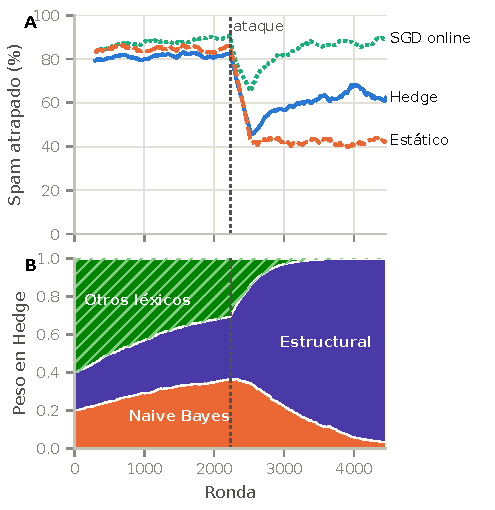
\includegraphics[width=\columnwidth]{f1f2_combinada.pdf}
\caption{A: spam atrapado en ventana móvil de 300 rondas. B: pesos de \emph{Hedge}; ``otros
léxicos'' agrupa regresión logística, árbol y reglas. Promedio de 20 semillas.}
\label{fig:pesos}
\end{figure}

\paragraph{Combinar o reentrenar.} El ataque lleva al estático de 85 a 42\,\% de spam atrapado y
destroza a los otros expertos léxicos (regresión logística 7\,\%, árbol 22\,\%, reglas 15\,\%); el
estructural pasa de 81 a 66\,\%. Reentrenar es lo que más recupera (Tabla~\ref{tab:competidores}),
como anticipan \citet{lowd2005goodword}. Pero \emph{Hedge}, sin tocar ningún modelo, cubre el
$47 \pm 13\,\%$ de la brecha entre el estático y SGD online (mediana 44\,\%, rango 23--76\,\%). La
Fig.~\ref{fig:pesos} muestra el mecanismo en dos partes. Al llegar el ataque el peso está repartido
en tercios (Naive Bayes 0,36, estructural 0,33, otros 0,31): \emph{Hedge} no apostó todo al mejor
del momento. Después, el estructural tarda unas 1.000 rondas en concentrar el peso, y el spam
atrapado sube con él desde $\approx 45\,\%$. Su techo es el del mejor experto fijo; SGD lo supera
porque aprende los tokens nuevos. El seguro tiene un costo: antes del ataque \emph{Hedge}
randomizado comete más errores que el estático (72 contra 60), precio de sortear expertos en lugar
de seguir al mejor, que el voto determinístico no paga.

\begin{figure}[t]
\centering
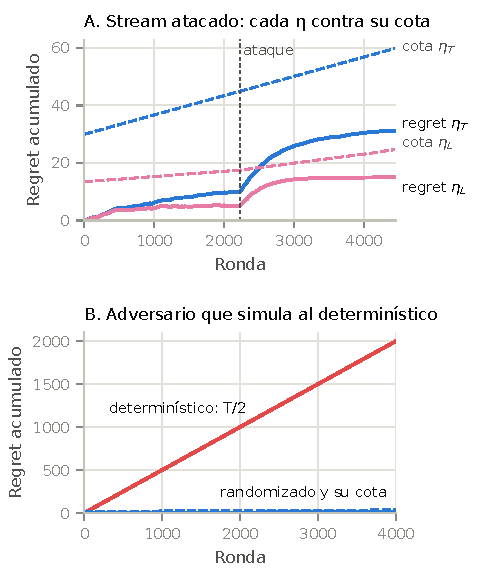
\includegraphics[width=\columnwidth]{f3_regret.pdf}
\caption{A: regret de \emph{Hedge} con $\etaT$ y con $\etaL$, cada uno contra su cota como curva en
el tiempo (media de 20 semillas). B: adversario que simula al jugador determinístico.}
\label{fig:regret}
\end{figure}

\paragraph{Garantías.} Con $\etaT$ el regret es $31,2 \pm 1,6$, bajo la cota~\eqref{eq:peorcaso} de
$59,9$ en las 20 semillas; con $\etaL$ baja a $15,0 \pm 1,4$, bajo su cota de $25,2$ en las 20. La
Fig.~\ref{fig:regret}A muestra la diferencia de forma: la cota de peor caso es una recta, mientras
que la de \citet{freund1997decision} aumenta su pendiente con el ataque, porque sigue la pérdida
acumulada del mejor experto. El análisis \emph{small-loss} no solo acota mejor: prescribe un
algoritmo mejor, al costo de una sintonía de oráculo. El voto determinístico, en cambio, tiene
regret $-2,6 \pm 4,8$ en el \emph{stream}: sobre una secuencia benigna le gana al mejor experto,
como cualquier ensamble, aunque en el peor caso no tiene garantía alguna (Fig.~\ref{fig:regret}B).

\begin{figure}[t]
\centering
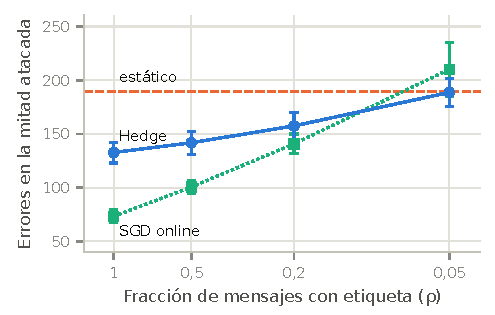
\includegraphics[width=\columnwidth]{f4_rho.pdf}
\caption{Errores en la mitad atacada según la fracción de mensajes etiquetados. Media $\pm$ desvío
entre 20 semillas; \emph{Hedge} y SGD ven las mismas rondas etiquetadas.}
\label{fig:rho}
\end{figure}

\paragraph{Etiqueta escasa.} Al bajar $\rho$, \emph{Hedge} se degrada de 132 a 188 errores y SGD de
73 a 210 (Fig.~\ref{fig:rho}). Con $\rho \ge 0,2$ reentrenar gana en 18 o más de las 20 semillas;
con $\rho = 0,05$ combinar gana en 16, y SGD termina peor que no adaptarse (210 contra 190 del
estático). La explicación es de conteo: para recuperarse, reentrenar tiene que aprender del orden de
un peso por token nuevo, mientras que \emph{Hedge} aprende $K = 5$. El regret de \emph{Hedge} escala
con pendiente $-0,37$ en escala log-log, contra $-0,5$ de la teoría; hasta $\rho = 0,2$ sigue bien
la ley $1/\sqrt{\rho}$, y con $\rho = 0,05$ satura al acercarse al regret de no aprender nunca
($143 \pm 21$, pesos uniformes siempre).

% ---------------------------------------------------------------------------
\section{Discusión y limitaciones}

El resultado matiza a \citet{lowd2005goodword}: reentrenar seguido funciona si hay etiquetas
seguido. Cuando escasean, combinar expertos fijos es más robusto, porque tiene muchos menos
parámetros que aprender.

La recuperación de \emph{Hedge} depende de que exista un experto que sobreviva al ataque, y lo
medimos: con una primera versión del experto estructural, de cinco rasgos y $\approx 30\,\%$ de
spam atrapado, \emph{Hedge} terminaba con 0,995 del peso en el estático dañado y no recuperaba nada
(en la semilla de desarrollo; esa versión no se corrió con las 20).
Nuestro experto robusto lo es por construcción; un ataque que ofuscara también teléfonos y tarifas
lo rompería. Además \emph{Hedge} no olvida: su garantía es contra el mejor experto \emph{fijo} en
todo el horizonte, y un experto con mucha pérdida acumulada tarda en recuperar peso. Aquí no pesa,
porque el estructural ya era competitivo antes del ataque; para el caso general, \emph{Fixed-Share}
compite contra el mejor experto por tramos~\cite{herbster1998tracking}.

Hay también una lección metodológica: la validación cruzada sobre un \emph{warm-up} sin drift no
sirve para elegir hiperparámetros de adaptación (el $\alpha$ de SGD), y habría desplegado como
modelo estático al experto robusto en 6 de 20 semillas, por azar.

Limitaciones: la pérdida 0-1 es simétrica, aunque bloquear un mensaje legítimo cuesta más que dejar
pasar spam (por eso se reportan SC y BH por separado); el corpus no tiene fechas, así que el orden y
el drift son sintéticos; el modelo de etiqueta parcial es de dos lados, cuando en la práctica solo se
ven los errores de los mensajes entregados; y un adversario adaptativo con memoria acotada
degradaría las tasas de $\sqrt{T}$ a $T^{2/3}$~\cite{cesabianchi2013switching}.

% ---------------------------------------------------------------------------
\section{Conclusión}

Frente a un spammer que se adapta, combinar clasificadores congelados con \emph{Hedge} recupera
casi la mitad de lo que recupera reentrenar, sin tocar ningún modelo. Y cuando las etiquetas
escasean, combinar supera a reentrenar: el remedio de reentrenar seguido necesita etiquetas
frecuentes.

{\small
\bibliographystyle{plainnat}
\bibliography{referencias}
}

\end{document}
